\chapter{Predict Water Body from Time-series High-Resolution Radar Satellite Images}
\label{chap-5-predict-from-sar-image}
\begin{ChapAbstract}
In this chapter, we would like to apply machine learning approach, especially deep learning, to predict the water body in the next future. We apply an extension on Long Short-Term Memory (LSTM), Conv-LSTM, to tackle problem. Conv-LSTM layer is not only take advantage from previous state-of-the-art approach in this kind of problems, Fully-Connected LSTM, but also very suitable to spatial-temporal data due to inherent convolutional structure. Because of the common things between water body and rainfall intensity in spatial and temporal information, we apply model from precipitation nowcasting problem to our prediction problem, modify about ways to train model, then Tri An Reservor is one more time selected to take experiment on. 

\end{ChapAbstract}

\section{Related Work}

% Time-series data prediction: Video / Precipitation Nowcasting.

Prediction (a.k.a. sequence prediction) is one of interesting fields in machine learning, in which the input (sequence data) contains an order on the observations and this order must be preserved while training model and making prediction.

\begin{figure}[h!]
	\centering
	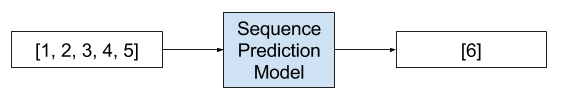
\includegraphics[width=0.7\textwidth]{figures/Example-of-a-Sequence-Prediction-Problem.png}
	\caption{Example of simple sequence prediction}
	\label{fig:exampleSimpleSequencePrediction}
\end{figure}

There are some example of sequence prediction problems, including:


\begin{enumerate}
	\item \textbf{Stock Market Prediction}\cite{Pagolu2016,Liu2018}. Given sequence of stock value as input, predict the expected next stock value. 
	
	\item \textbf{Product Recommendation}\cite{Wang2018,Cao2019}. Given sequence of recent purchased goods of a customer, predict the thing that the customer might "add to cart" next, and then make recommendation. 
	
	\item \textbf{Weather Forecasting}\cite{Quan2000,Wang2017}. Given sequence of weather observation over a period of time, predict the expected weather in next point of time.
	
\end{enumerate}

% Related to water body from satellite images, figure out why it related and its expansion: periodical information

One of important fields of weather forecasting is Nowcasting Precipitation\cite{Sun2013}. The goal of this task is about giving precise prediction of rainfall intensity in a region, over a short period of time. Recent advances in deep learning, Recurrent Neural Networks (RNNs), especially Long Short-Term Memories (LSTMs) models\cite{Graves2013GeneratingSW,Hochreiter1997,Cho2014,Donahue2017} provides good results on this kind of problem. In this thesis, we would like to predict the next water body shape (related to its area), from its time-series data. The common things between nowcasting precipitation and this problem is they both have spatial, spectral and temporal information inside data. We would like to apply model containing Conv-LSTM-2D layer\cite{Shi2015ConvolutionalLN}, to solve our proposed problem. Conv-LSTM-2D layer is recently used in computer vision, especially spatial-temporal problems. In this problem, we would like to extract the spatial feature as well as the correlation in the time. The fully-connected LSTMs can capture the temporal correlation but do not encode the spatial data. That's why they propose a model where the input to state and state to state transitions are convolutional. The model in \cite{Shi2015ConvolutionalLN} show better result on capturing spatial-temporal correlations than other state-of-the-art methods. So in this thesis, we will take this model as reference to provide solution for our problem, for Tri An reservoir.

\section{Dataset} 

In this chapter, Tri An reservoir is chosen for experiments. Because Radar Satellites Images is not affected by cloud cover like optical satellite in \ref{chap-3-recover-water-body}, so we only focus on prediction water body. The synthetic-aperture radar \footnote{https://en.wikipedia.org/wiki/Synthetic-aperture\_radar} monthly imagery provided from Sentinel-1 satellites \footnote{https://sentinel.esa.int/web/sentinel/missions/sentinel-1} are collected from \textit{November 25tr, 2015} to \textit{June 1st, 2019} for training and evaluating. 

Depending on coordinates of Tri An Reservoir, the original image has been cropped to size \textit{2560 px} x \textit{3840 px}, enough to show its water body.

\subsection{Water body segmentation on Sentinel-1 Image}

Sentinel-1 Satellite provides image with 10m spatial resolution. In this thesis, in order to segment out water body, we depend on VH or VV polarizations imagery and apply corresponding threshold:

\begin{equation}
\centering
VH \leq -21
\end{equation} 

\begin{equation}
\centering
VV \leq -17
\end{equation} 

Because in our cropped image that only contains Tri An Reservoir as the largest water body, so we only need to find out the most largest one, using Bread-First Search algorithm\footnote{https://en.wikipedia.org/wiki/Breadth-first\_search}. With this object, we easily to figure out the boundaries, with help of function \textit{find\_boundaries}, from Python library \textit{Scikit-Image}\footnote{https://scikit-image.org/}.

\section{Model}

The model has been implemented by Keras. Its structure is shown below:

\begin{figure}[h!]
	\centering
	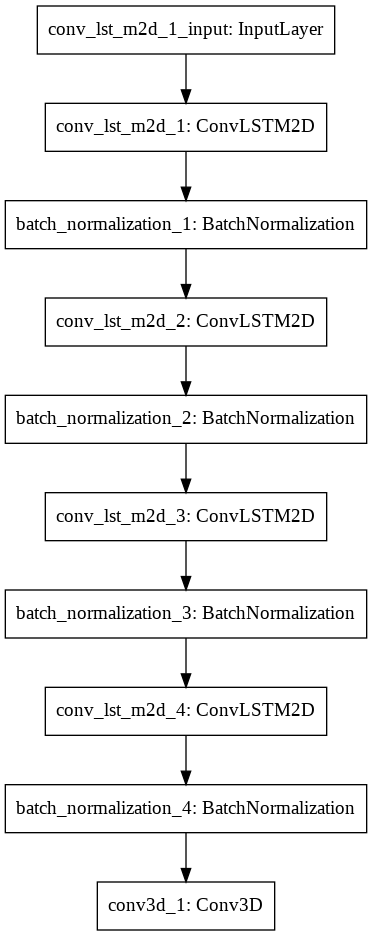
\includegraphics[width=0.5\textwidth]{figures/time_model.png}
	\caption{Prediction mode, based on Conv-LSTM-2D}
	\label{fig:timeModel}
\end{figure}

Model summary detail:

\begin{verbatim}
_________________________________________________________________
Layer (type)                 Output Shape               Param #   
=================================================================
conv_lst_m2d_1 (ConvLSTM2D)  (None, None, 128, 128, 64) 815616    
_________________________________________________________________
batch_normalization_1 (Batch (None, None, 128, 128, 64) 256       
_________________________________________________________________
conv_lst_m2d_2 (ConvLSTM2D)  (None, None, 128, 128, 32) 602240    
_________________________________________________________________
batch_normalization_2 (Batch (None, None, 128, 128, 32) 128       
_________________________________________________________________
conv_lst_m2d_3 (ConvLSTM2D)  (None, None, 128, 128, 32) 401536    
_________________________________________________________________
batch_normalization_3 (Batch (None, None, 128, 128, 32) 128       
_________________________________________________________________
conv_lst_m2d_4 (ConvLSTM2D)  (None, None, 128, 128, 32) 401536    
_________________________________________________________________
batch_normalization_4 (Batch (None, None, 128, 128, 32) 128       
_________________________________________________________________
conv3d_1 (Conv3D)            (None, None, 128, 128, 1)  33        
=================================================================
Total params: 2,221,601
Trainable params: 2,221,281
Non-trainable params: 320
_________________________________________________________________
\end{verbatim}

Specification:

\begin{itemize}
	\item \textit{Input and Output} Because we only focus on predicting water body, so after extracting water body from original image and finding out its boundaries, we randomize on boundaries 50 tiles with size of 128 x 128. There is 12 consecutive images, corresponding to 12 month in year. The output is a image of next month, which is same month of 1st image in input sequence but next year. 
	
	\item \textit{Conv3D} This type of layer helps to catch spatial and temporal invariances in the same manner as \textit{Conv2D} in an imagery case. This make the curse of dimensionality much less harmful. Because at the end of model, we need to have a prediction, so it's no longer to keep temporal information after this layer.
	
	\item \textit{Batch Normalization} Batch normalization reduces the amount by what the hidden unit values shift around (covariance shift). Morever, this layer allows each layer of a network to learn by itself a little bit more independently of other layers.
	
	\item \textit{Activation} The activation for Conv-LSTM-2D is $tanh$ function, for Conv3D is $sigmoid$ function.
	
	\item \textit{Dropout and Recurrent Dropout} In Recurrent Neural Networks, we have two definition about \textbf{Dropout} and \textbf{Recurrent Dropout}. \textbf{Dropout} describes fraction of the units to drop for the linear transformation of the inputs, while \textbf{Recurrent Dropout} show fraction of the units to drop for the linear transformation of the recurrent state (more detail at \cite{Gal2015}). In this model, with each Conv-LSTM-2D layer's configuration, $dropout$ is set at $0.4$, and and $recurrent\_dropout$ is $0.3$.
	
	\item \textit{Model compilation parameters} Like model compilation in \ref{chap-3-recover-water-body}, the loss function is still $mean_square_error$, optimizer is $adam$ and evaluation metric is $PSNR$(\ref{psnr_eq}). 
	
\end{itemize}

\section{Experiments}

\subsection{Prediction water body area}

% Show demo 12 input in 1 line

% Show table, contains result

% Plot predicted result, with groundtruth value

% Show 2-6/19 prediction, with result and boundaries.

\subsection{Anomaly sample}

% Plot anomaly in previous time

% Show image

% etc...



\section{Conclusions}

